% Created 2020-05-05 Tue 21:20
% Intended LaTeX compiler: pdflatex
\documentclass[11pt]{article}
\usepackage[utf8]{inputenc}
\usepackage[T1]{fontenc}
\usepackage{graphicx}
\usepackage{grffile}
\usepackage{longtable}
\usepackage{wrapfig}
\usepackage{rotating}
\usepackage[normalem]{ulem}
\usepackage{amsmath}
\usepackage{textcomp}
\usepackage{amssymb}
\usepackage{capt-of}
\usepackage{hyperref}
\date{\today}
\title{}
\hypersetup{
 pdfauthor={},
 pdftitle={},
 pdfkeywords={},
 pdfsubject={},
 pdfcreator={Emacs 26.3 (Org mode 9.3.6)},
 pdflang={English}}
\begin{document}

\tableofcontents

\section{Meetings}
\label{sec:org67b957e}
\subsection{{\bfseries\sffamily DONE} Meeting with Dr Amber}
\label{sec:org9b91afc}
Participants:
\begin{itemize}
\item Dr Ityonna Amber
\item Vi Kumar
\end{itemize}

\subsection{{\bfseries\sffamily DONE} Meeting}
\label{sec:orgc07af9a}
Participants:
\begin{itemize}
\item Dr Ityonna Amber
\item Dr Mehdi Nazarinia
\item Sherrif Abdullah
\item Vi Kumar
\end{itemize}

Little more than second year knowledge required but should be fun.
Control Scheme is hardest part BUT that's the crux of the competition.

\subsubsection{Action items summary}
\label{sec:org1d754ce}
\begin{itemize}
\item Finish Onramp training and get software installed and ready
\item Lookup previous years drones and results
\begin{itemize}
\item Research about drone line-followers would be nice
\end{itemize}
\item Background Research on Control Theory
\begin{itemize}
\item Definitely a bit on the practical side since trusting EEs to make theory simple is a bad move.
\end{itemize}
\end{itemize}

\subsection{{\bfseries\sffamily TODO} Meeting}
\label{sec:orgacf31a4}
Participants:
\begin{itemize}
\item Dr Ityonna Amber
\item Dr Mehdi Nazarinia
\item Sherrif Abdullah
\item Vi Kumar
\end{itemize}

Decide then whether to have weekly or biweekly meetings

\section{Competition\hfill{}\textsc{slide}}
\label{sec:org5e75a20}
Email: roboticsarena@mathworks.com

Round 1 - Simulation in Simulink
Round 2 - Deployment Round on Parrot Mambo Minidrone

\subsection{Timeline\hfill{}\textsc{slide}}
\label{sec:org5faaa89}

\begin{center}
\begin{tabular}{ll}
Competition launch & 03 Feb 2020\\
Round 1 application closure & 06 July 2020, 6 PM BST\\
Round 1 submission & 27 July 2020\\
Round 1 result declaration & 01 Sept 2020\\
Round 2 live event and winners & 01 Oct 2020\\
\end{tabular}
\end{center}

\subsubsection{Submit application}
\label{sec:org339af3d}
Should be as simple as sending in a list of names.

\subsubsection{Round 1 - Simulation in Simulink}
\label{sec:org9e6fe04}
Simulink model is submitted.

Submitted models are graded on:
\begin{itemize}
\item Accuracy of the traced path
\item Time taken to complete track
\item Successful landing on end marker
\item NOTE Code generation is required.
\item NOTE Multiple evaluation passes are done by Mathworks Engineers
\end{itemize}

\subsubsection{Round 2 - Deployment Round}
\label{sec:orgd4063c9}
\textit{<2020-04-26 Sun>}
Somewhat uncertain due to the whole coronavirus lockdown.
Probably going to be a virtual thing. \textasciitilde{}Dr Mehdi

Practice Round
\begin{itemize}
\item not evaluated
\item two slots of 15 minutes
\item Calibrate and test algorithms
\end{itemize}

Live Round
\begin{itemize}
\item one 15-minute slot
\item Seven chances to run the hardware
\item Nomination of one chance.
\item Graded based on number of track sections completed.
\item Judges decide which stages are considered complete.
\end{itemize}

\subsection{Software Requirements\hfill{}\textsc{slide}}
\label{sec:org0253270}
\begin{itemize}
\item Latest version of Matlab
\item Optional Simulink OnRamp
\item Simulink Package for ParrotDrone
\begin{itemize}
\item Allows you to deploy simulink models to Parrot Drone
\end{itemize}
\end{itemize}

\subsubsection{{\bfseries\sffamily TODO} OnRamp Online Courses}
\label{sec:org3bd7591}
Finish it for the minimum training required for the competition.
\begin{itemize}
\item Matlab Onramp
\item Simulink Onramp
\item Stateflow Onramp
\end{itemize}

Work w/ Abdullah on this. Should be doable by next meeting.
Definitely need to keep track of it.

\subsubsection{{\bfseries\sffamily WAITING} Simulink Package Configuration}
\label{sec:org5124b88}
Bluetooth issues for Windows (Send the online help page to Dr Mehdi)
Hardware Deployment Issues

NOTE: Need to try simulation before actually figuring hardware issues

\subsection{{\bfseries\sffamily TODO} Control Schemes}
\label{sec:org4e3c594}
with drone context

Work w/ Abdullah on this.
Need to make a plan for next steps.

\subsection{{\bfseries\sffamily DONE} Create a Microsoft Teams group}
\label{sec:org82f593f}
\subsubsection{{\bfseries\sffamily DONE} Upload some basic information about the competition}
\label{sec:org8885332}
Competition rules and this doc.
\subsection{Mission objective\hfill{}\textsc{slide}}
\label{sec:orgf695192}

\begin{itemize}
\item Take off from a circular pad
\item Follow a track laid on floor
\begin{itemize}
\item Track sections have straight lines with no curves
\item Downward facing camera to track lines
\end{itemize}
\item Land on circular end marker

Time considered only when the minidrone lands on the end marker.
In order for the minidrone to be considered as having landed:
\begin{itemize}
\item Minidrone must be upright.
\item Minidrone's bottom surface has to touch the floor.
\end{itemize}
\begin{center}
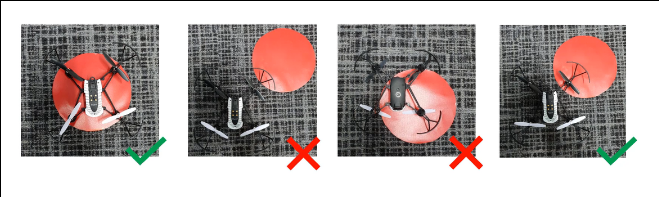
\includegraphics[width=.9\linewidth]{./images/screenshot-01.png}
\end{center}
\end{itemize}

\section{Parrot Mambo Drone General info\hfill{}\textsc{slide}}
\label{sec:org2dbfb8a}
\subsection{Miscellaneous}
\label{sec:org1f0a261}
\subsubsection{Energy}
\label{sec:orgfacc3f3}
660mAh LiPo Battery
8 min autonomy with accessory connected or bumpers
10 min autonomy with neither accessory nor bumpers
30 min charging time with a 2,1A charger

\subsubsection{SDK}
\label{sec:orga233967}
SDK: OS Linux. SDK available on Parrot.com
We might find documentation useful, especially if the Simulink model neglects to mention something.

\subsection{Sensors}
\label{sec:org870641d}
\subsubsection{Stabilization sensors :}
\label{sec:org2df710e}
Inertial Measurement Unit to evaluate speed, tilt and obstacle contact (3-axis accelerometer and 3-axis gyroscope)
Ultrasound sensor
Pressure sensor
Camera sensor

\subsubsection{Speed measurement :}
\label{sec:org78cc47d}
60 FPS vertical camera
120x160 pixel resolution
Ultrasound sensor

\subsubsection{Streaming Camera}
\label{sec:org6a1847e}
Streaming and Recording HD 720p 30 FPS
FOV 120°
\begin{center}
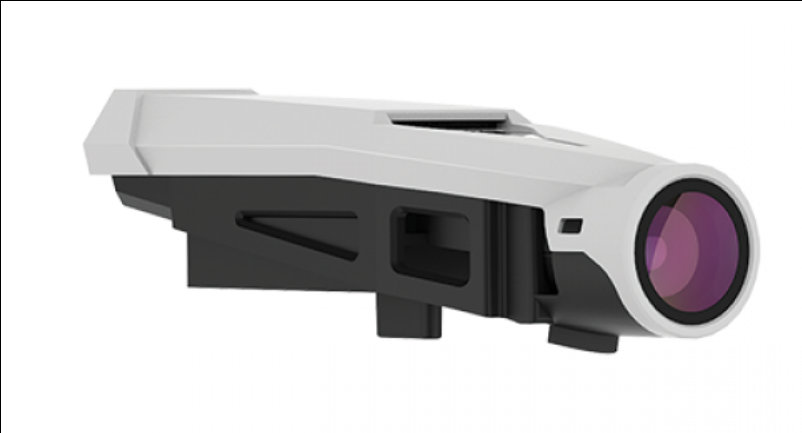
\includegraphics[width=.9\linewidth]{./images/screenshot-02.png}
\end{center}i

\begin{center}
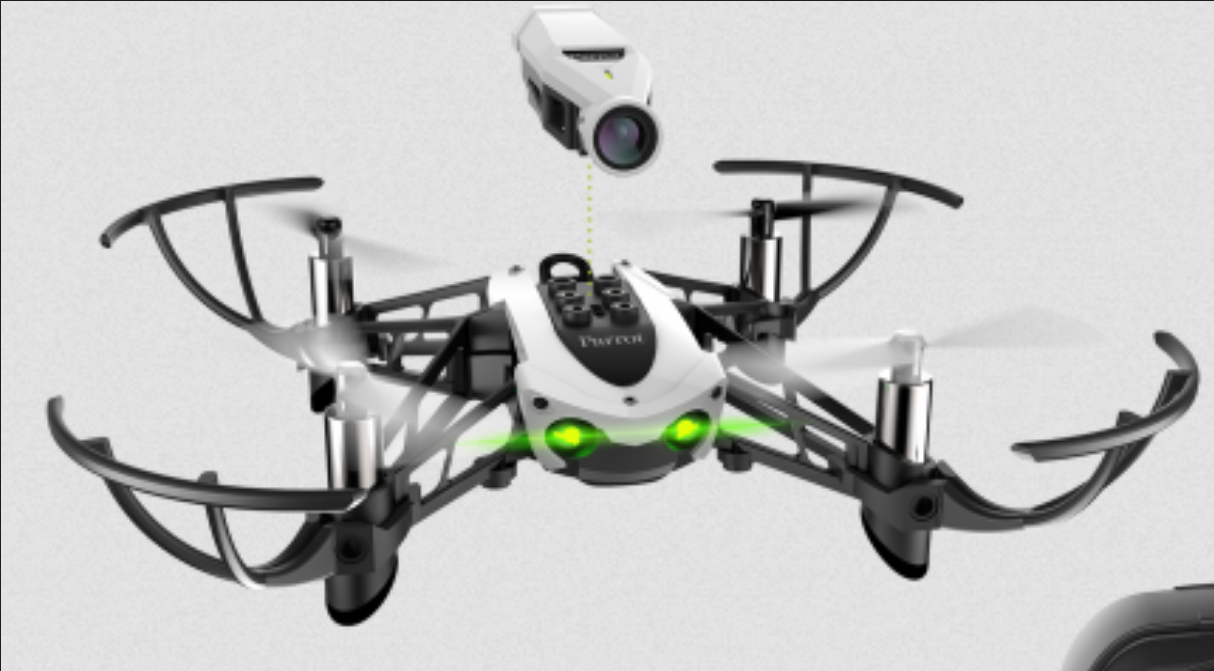
\includegraphics[width=.9\linewidth]{./images/screenshot-03.png}
\end{center}

\subsection{Physical Characteristics}
\label{sec:org2d9f1d2}
Need to get a MoI matrix from this
\subsubsection{Weight :}
\label{sec:org8572236}
Weight: 2.22 oz / 63g (without bumpers or accessories)
Weight with Camera: 73g
\subsubsection{Dimensions}
\label{sec:org5b92d0e}
7.1 x 7.1 in. / 18 x 18 cm with Bumpers
\subsubsection{Rotor Characteristics}
\label{sec:org75abfd6}

\begin{center}
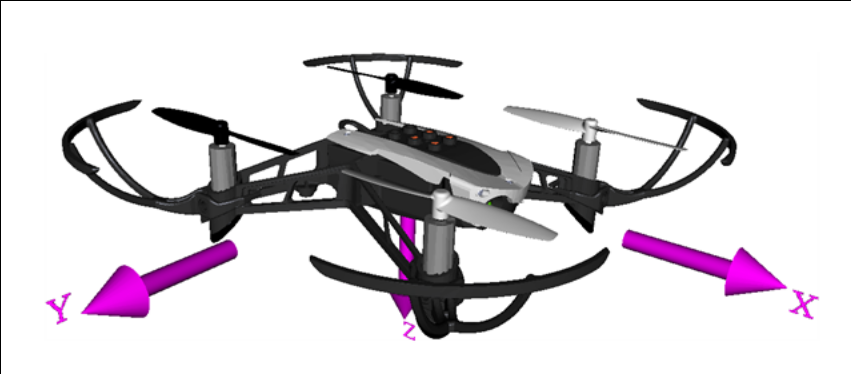
\includegraphics[width=.9\linewidth]{./images/screenshot-04.png}
\end{center}

Right-hand Coordinate Frame centered at Center of gravity.

Rotor \#1 rotates positively with respect to the z-axis. It is located parallel to the xy-plane, -45 degrees from the x-axis.

Rotor \#2 rotates negatively with respect to the body's z-axis. It is located parallel to the xy-plane, -135 degrees from the x-axis.

Rotor \#3 has the same rotation direction as rotor \#1. It is located parallel to the xy-plane, 135 degrees from the x-axis.

Rotor \#4 has the same rotation direction as rotor \#2. It is located parallel to the xy-plane, 45 degrees from the x-axis.

\section{Control\hfill{}\textsc{slide}}
\label{sec:org58a2a5f}
\subsection{Simulink Model Description}
\label{sec:orgbdc0dc7}

\begin{itemize}
\item flight Control system
\item Image processing
\begin{itemize}
\item Loads of OpenCV-like filters
\item Rate Transition since control system runs faster than image processing
\begin{itemize}
\item Any way to create multiple buffers for image processing?
This would allow much better "time resolution"
\end{itemize}
\end{itemize}
\item Drone Controller
\begin{itemize}
\item Real-time measurement
\end{itemize}
\item Control path planning algorithm
\end{itemize}

\subsubsection{{\bfseries\sffamily TODO} Sensor Filter}
\label{sec:org7e95304}
Extended Kalman Feedback is what I'm familiar with BUT
\begin{itemize}
\item it's a linear filter, how does it deal with a drone's non-linearities?
Kalman filters assume Gaussian noise on "true" values that are linear-ish
How accurate is this model?
\item Is it even worthwhile to bother with it is a simpler scheme works?
\end{itemize}
\begin{enumerate}
\item {\bfseries\sffamily TODO} How to use vision-based feedback in the correction step?
\label{sec:org2d0a8bf}
Vision-based odometry is apparently a thing for drones.

Contact Dr Mehdi \& Dr Tadhg for vision processing and path planning. \textasciitilde{}Dr Amber

Definitely need to figure out how to use the data after we've manipulated the raw data from the drone camera.
\end{enumerate}

\subsubsection{{\bfseries\sffamily TODO} Control Schemes}
\label{sec:org8240aad}
To be researched. But really need value judgements from a human.

\begin{itemize}
\item PID
\item Fuzzy PID
\item LQR
\item LQG/LTR
\item H-infinity
\item Loop Shaping
\item MPC
\end{itemize}

Perhaps a silly question, can we improve upon a previous run for a given track?
How can we use existing data to contruct a "true-er" model from a previous run (especially at section junction)

\subsection{Sensor Hardware \& Related thoughts}
\label{sec:org8db1624}
\subsubsection{Inertial Measurement Unit (IMU)}
\label{sec:org349b6f4}
Inertial Measurement Unit to evaluate speed, tilt and obstacle contact
\begin{itemize}
\item 3-axis accelerometer
\item 3-axis gyroscope
\end{itemize}

Definitely need to get accurate specs for this.
The Parrot AR Drone had pretty good IMU chips so pretty sure that even a "low-cost" model should have something with:
\begin{itemize}
\item accelerometer +-2g
\item Bandwidth \textasciitilde{}1000Hz
\item Low cross-axis misalignment
\end{itemize}

Not sure how Mathworks's Simulink package deals with the hardware flags but should be interesting to see.

\begin{enumerate}
\item Accelerometer Characterization
\label{sec:org7251a69}
\begin{itemize}
\item Bias factor
\item Scale factor
\item Thermal drift (check if it's relevant? Should be a simple correction)
\end{itemize}
\end{enumerate}

\subsubsection{Downward facing Camera}
\label{sec:org7fdcce9}
60 FPS vertical camera
120x160 pixel resolution

Located near COG and next to the ultrasound sensor.

\begin{itemize}
\item Do we need to worry about the actual picture being distorted?
OpenCV has a little camera calibration thingy that takes care of camera distortion.
A chessboard pattern? Something similar here would be sweet.

\item How do we detect the red path and convert it to a line path?
More of a question for the control scheme but should keep in mind.
\end{itemize}

\begin{enumerate}
\item How to do the binary switch for on-off image processing
\label{sec:org1248156}

canny edge to hough processing

canny edge to hough processing

do it for submission

move towards code that focuses on deviation from the center.

Ask Dr Mehdi for help with Mathworks documentations
\end{enumerate}


\section{Image processing summary}
\label{sec:orgf472584}

canny edge > hough transform

inaccuracy in the image or just plain ol' reliability

Also need to figure out if there are better methods out there.

test suite of red track on carpet.

Spepd of camera and te type of communication for the same

FPV camera to predict future paths as well

\section{Application}
\label{sec:orgd23839b}

\begin{itemize}
\item Code generation

\item Forth year and Third year examinations.
\item Sample images from Dr Mehsi after that.

\item 17th Sunday
\end{itemize}
\end{document}
